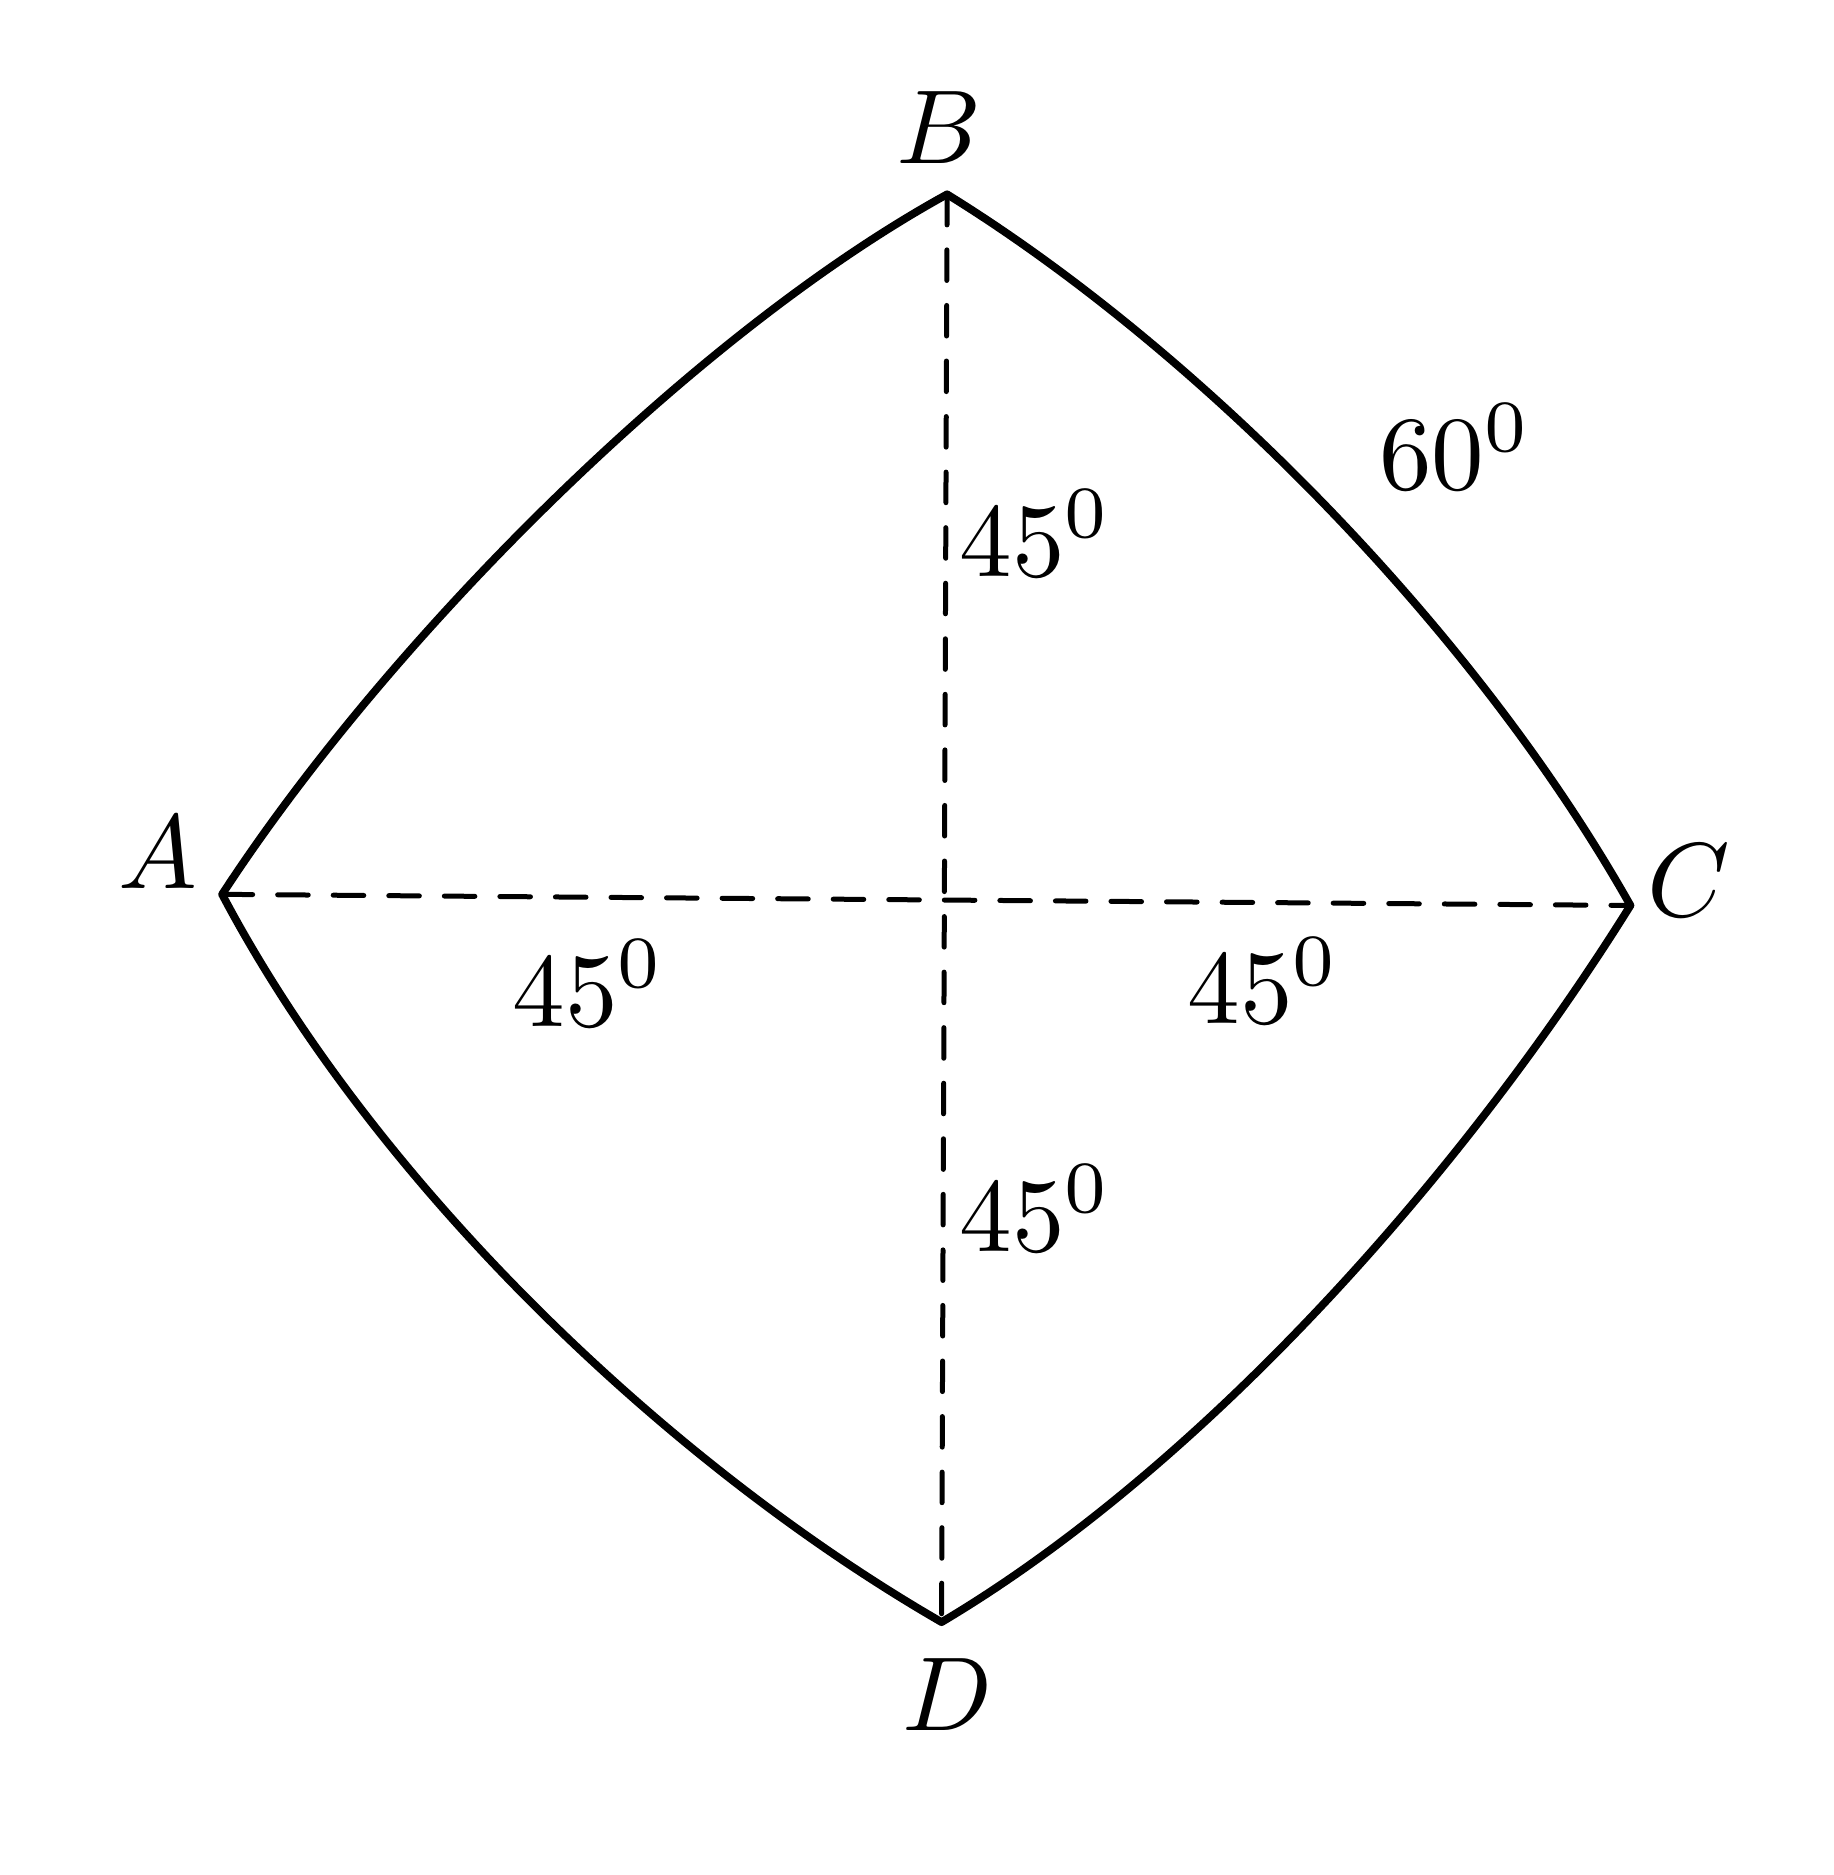
\begin{tikzpicture}[x=1bp,y=-1bp,line cap=round,line join=round]
\path[use as bounding box] (0,0) rectangle (640,655);
\begin{pgfinterruptboundingbox}
\draw[line width=2.8bp] (70,312) .. controls (130,220) and (240,110) .. (331,60) .. controls (420,115) and (520,215) .. (577,316) .. controls (514,417) and (420,520) .. (329,574) .. controls (232,518) and (126,418) .. (70,312);
\draw[line width=1.8bp,dash pattern=on 11bp off 9bp] (70,312) -- (577,316);
\draw[line width=1.8bp,dash pattern=on 11bp off 9bp] (331,60) -- (329,574);
\node[inner sep=0pt,outer sep=0pt] at (47,297) {\scalebox{3.8}{\ensuremath{A}}};
\node[inner sep=0pt,outer sep=0pt] at (328,36) {\scalebox{3.8}{\ensuremath{B}}};
\node[inner sep=0pt,outer sep=0pt] at (598,307) {\scalebox{3.8}{\ensuremath{C}}};
\node[inner sep=0pt,outer sep=0pt] at (331,600) {\scalebox{3.8}{\ensuremath{D}}};
\node[inner sep=0pt,outer sep=0pt] at (363,182) {\scalebox{3.8}{\ensuremath{45^0}}};
\node[inner sep=0pt,outer sep=0pt] at (445,343) {\scalebox{3.8}{\ensuremath{45^0}}};
\node[inner sep=0pt,outer sep=0pt] at (363,425) {\scalebox{3.8}{\ensuremath{45^0}}};
\node[inner sep=0pt,outer sep=0pt] at (202,344) {\scalebox{3.8}{\ensuremath{45^0}}};
\node[inner sep=0pt,outer sep=0pt] at (514,151) {\scalebox{3.8}{\ensuremath{60^0}}};
\end{pgfinterruptboundingbox}
\end{tikzpicture}
